\documentclass{beamer}

\usetheme{Warsaw}
\usepackage{graphicx}
\usepackage{ulem}
% include.tex
\newcommand{\Bernoulli}[1]{\text{Bernoulli} \left( #1 \right)}
\newcommand{\mydigamma}[1]{\psi \left( #1 \right)}
%\newcommand{\diag}[1]{\text{diag}\left( #1 \right)}
\newcommand{\tr}[1]{\text{tr}\left( #1 \right)}
\newcommand{\Poisson}[1]{\text{Poisson} \left( #1 \right)}
\def \half {\frac{1}{2}}
\def \R {\mathbb{R}}
\def \vbeta {\vec{\beta}}
\def \vy {\vec{y}}
\def \vmu {\vec{\mu}}
\def \vmuqbeta {\vmu_{q(\vbeta)}}
\def \vmubeta {\vmu_{\vbeta}}
\def \Sigmaqbeta {\Sigma_{q(\vbeta)}}
\def \Sigmabeta {\Sigma_{\vbeta}}
\def \va {\vec{a}}
\def \vtheta {\vec{\theta}}
\def \mX {\vec{X}}

\def\ds{{\displaystyle}}

\def\diag{{\mbox{diag}}}


\usepackage{latexsym,amssymb,amsmath,amsfonts}
%\usepackage{tabularx}
\usepackage{theorem}
\usepackage{verbatim,array,multicol,palatino}
\usepackage{graphicx}
\usepackage{graphics}
\usepackage{fancyhdr}
\usepackage{algorithm,algorithmic}
\usepackage{url}
%\usepackage[all]{xy}



\def\approxdist{\stackrel{{\tiny \mbox{approx.}}}{\sim}}
\def\smhalf{\textstyle{\frac{1}{2}}}
\def\vxnew{\vx_{\mbox{{\tiny new}}}}
\def\bib{\vskip12pt\par\noindent\hangindent=1 true cm\hangafter=1}
\def\jump{\vskip3mm\noindent}
\def\etal{{\em et al.}}
\def\etahat{{\widehat\eta}}
\def\thick#1{\hbox{\rlap{$#1$}\kern0.25pt\rlap{$#1$}\kern0.25pt$#1$}}
\def\smbbeta{{\thick{\scriptstyle{\beta}}}}
\def\smbtheta{{\thick{\scriptstyle{\theta}}}}
\def\smbu{{\thick{\scriptstyle{\rm u}}}}
\def\smbzero{{\thick{\scriptstyle{0}}}}
\def\boxit#1{\begin{center}\fbox{#1}\end{center}}
\def\lboxit#1{\vbox{\hrule\hbox{\vrule\kern6pt
      \vbox{\kern6pt#1\kern6pt}\kern6pt\vrule}\hrule}}
\def\thickboxit#1{\vbox{{\hrule height 1mm}\hbox{{\vrule width 1mm}\kern6pt
          \vbox{\kern6pt#1\kern6pt}\kern6pt{\vrule width 1mm}}
               {\hrule height 1mm}}}


%\sloppy
%\usepackage{geometry}
%\geometry{verbose,a4paper,tmargin=20mm,bmargin=20mm,lmargin=40mm,rmargin=20mm}


%%%%%%%%%%%%%%%%%%%%%%%%%%%%%%%%%%%%%%%%%%%%%%%%%%%%%%%%%%%%%%%%%%%%%%%%%%%%%%%%
%
% Some convenience definitions
%
% \bf      -> vector
% \sf      -> matrix
% \mathcal -> sets or statistical
% \mathbb  -> fields or statistical
%
%%%%%%%%%%%%%%%%%%%%%%%%%%%%%%%%%%%%%%%%%%%%%%%%%%%%%%%%%%%%%%%%%%%%%%%%%%%%%%%%

% Sets or statistical values
\def\sI{{\mathcal I}}                            % Current Index set
\def\sJ{{\mathcal J}}                            % Select Index set
\def\sL{{\mathcal L}}                            % Likelihood
\def\sl{{\ell}}                                  % Log-likelihood
\def\sN{{\mathcal N}}                            
\def\sS{{\mathcal S}}                            
\def\sP{{\mathcal P}}                            
\def\sQ{{\mathcal Q}}                            
\def\sB{{\mathcal B}}                            
\def\sD{{\mathcal D}}                            
\def\sT{{\mathcal T}}
\def\sE{{\mathcal E}}                            
\def\sF{{\mathcal F}}                            
\def\sC{{\mathcal C}}                            
\def\sO{{\mathcal O}}                            
\def\sH{{\mathcal H}} 
\def\sR{{\mathcal R}}                            
\def\sJ{{\mathcal J}}                            
\def\sCP{{\mathcal CP}}                            
\def\sX{{\mathcal X}}                            
\def\sA{{\mathcal A}} 
\def\sZ{{\mathcal Z}}                            
\def\sM{{\mathcal M}}                            
\def\sK{{\mathcal K}}     
\def\sG{{\mathcal G}}                         
\def\sY{{\mathcal Y}}                         
\def\sU{{\mathcal U}}  


\def\sIG{{\mathcal IG}}                            


\def\cD{{\sf D}}
\def\cH{{\sf H}}
\def\cI{{\sf I}}

% Vectors
\def\vectorfontone{\bf}
\def\vectorfonttwo{\boldsymbol}
\def\va{{\vectorfontone a}}                      %
\def\vb{{\vectorfontone b}}                      %
\def\vc{{\vectorfontone c}}                      %
\def\vd{{\vectorfontone d}}                      %
\def\ve{{\vectorfontone e}}                      %
\def\vf{{\vectorfontone f}}                      %
\def\vg{{\vectorfontone g}}                      %
\def\vh{{\vectorfontone h}}                      %
\def\vi{{\vectorfontone i}}                      %
\def\vj{{\vectorfontone j}}                      %
\def\vk{{\vectorfontone k}}                      %
\def\vl{{\vectorfontone l}}                      %
\def\vm{{\vectorfontone m}}                      % number of basis functions
\def\vn{{\vectorfontone n}}                      % number of training samples
\def\vo{{\vectorfontone o}}                      %
\def\vp{{\vectorfontone p}}                      % number of unpenalized coefficients
\def\vq{{\vectorfontone q}}                      % number of penalized coefficients
\def\vr{{\vectorfontone r}}                      %
\def\vs{{\vectorfontone s}}                      %
\def\vt{{\vectorfontone t}}                      %
\def\vu{{\vectorfontone u}}                      % Penalized coefficients
\def\vv{{\vectorfontone v}}                      %
\def\vw{{\vectorfontone w}}                      %
\def\vx{{\vectorfontone x}}                      % Covariates/Predictors
\def\vy{{\vectorfontone y}}                      % Targets/Labels
\def\vz{{\vectorfontone z}}                      %

\def\vone{{\vectorfontone 1}}
\def\vzero{{\vectorfontone 0}}

\def\valpha{{\vectorfonttwo \alpha}}             %
\def\vbeta{{\vectorfonttwo \beta}}               % Unpenalized coefficients
\def\vgamma{{\vectorfonttwo \gamma}}             %
\def\vdelta{{\vectorfonttwo \delta}}             %
\def\vepsilon{{\vectorfonttwo \epsilon}}         %
\def\vvarepsilon{{\vectorfonttwo \varepsilon}}   % Vector of errors
\def\vzeta{{\vectorfonttwo \zeta}}               %
\def\veta{{\vectorfonttwo \eta}}                 % Vector of natural parameters
\def\vtheta{{\vectorfonttwo \theta}}             % Vector of combined coefficients
\def\vvartheta{{\vectorfonttwo \vartheta}}       %
\def\viota{{\vectorfonttwo \iota}}               %
\def\vkappa{{\vectorfonttwo \kappa}}             %
\def\vlambda{{\vectorfonttwo \lambda}}           % Vector of smoothing parameters
\def\vmu{{\vectorfonttwo \mu}}                   % Vector of means
\def\vnu{{\vectorfonttwo \nu}}                   %
\def\vxi{{\vectorfonttwo \xi}}                   %
\def\vpi{{\vectorfonttwo \pi}}                   %
\def\vvarpi{{\vectorfonttwo \varpi}}             %
\def\vrho{{\vectorfonttwo \rho}}                 %
\def\vvarrho{{\vectorfonttwo \varrho}}           %
\def\vsigma{{\vectorfonttwo \sigma}}             %
\def\vvarsigma{{\vectorfonttwo \varsigma}}       %
\def\vtau{{\vectorfonttwo \tau}}                 %
\def\vupsilon{{\vectorfonttwo \upsilon}}         %
\def\vphi{{\vectorfonttwo \phi}}                 %
\def\vvarphi{{\vectorfonttwo \varphi}}           %
\def\vchi{{\vectorfonttwo \chi}}                 %
\def\vpsi{{\vectorfonttwo \psi}}                 %
\def\vomega{{\vectorfonttwo \omega}}             %


% Matrices
%\def\matrixfontone{\sf}
%\def\matrixfonttwo{\sf}
\def\matrixfontone{\bf}
\def\matrixfonttwo{\boldsymbol}
\def\mA{{\matrixfontone A}}                      %
\def\mB{{\matrixfontone B}}                      %
\def\mC{{\matrixfontone C}}                      % Combined Design Matrix
\def\mD{{\matrixfontone D}}                      % Penalty Matrix for \vu_J
\def\mE{{\matrixfontone E}}                      %
\def\mF{{\matrixfontone F}}                      %
\def\mG{{\matrixfontone G}}                      % Penalty Matrix for \vu
\def\mH{{\matrixfontone H}}                      %
\def\mI{{\matrixfontone I}}                      % Identity Matrix
\def\mJ{{\matrixfontone J}}                      %
\def\mK{{\matrixfontone K}}                      %
\def\mL{{\matrixfontone L}}                      % Lower bound
\def\mM{{\matrixfontone M}}                      %
\def\mN{{\matrixfontone N}}                      %
\def\mO{{\matrixfontone O}}                      %
\def\mP{{\matrixfontone P}}                      %
\def\mQ{{\matrixfontone Q}}                      %
\def\mR{{\matrixfontone R}}                      %
\def\mS{{\matrixfontone S}}                      %
\def\mT{{\matrixfontone T}}                      %
\def\mU{{\matrixfontone U}}                      % Upper bound
\def\mV{{\matrixfontone V}}                      %
\def\mW{{\matrixfontone W}}                      % Variance Matrix i.e. diag(b'')
\def\mX{{\matrixfontone X}}                      % Unpenalized Design Matrix/Nullspace Matrix
\def\mY{{\matrixfontone Y}}                      %
\def\mZ{{\matrixfontone Z}}                      % Penalized Design Matrix/Kernel Space Matrix

\def\mGamma{{\matrixfonttwo \Gamma}}             %
\def\mDelta{{\matrixfonttwo \Delta}}             %
\def\mTheta{{\matrixfonttwo \Theta}}             %
\def\mLambda{{\matrixfonttwo \Lambda}}           % Penalty Matrix for \vnu
\def\mXi{{\matrixfonttwo \Xi}}                   %
\def\mPi{{\matrixfonttwo \Pi}}                   %
\def\mSigma{{\matrixfonttwo \Sigma}}             %
\def\mUpsilon{{\matrixfonttwo \Upsilon}}         %
\def\mPhi{{\matrixfonttwo \Phi}}                 %
\def\mOmega{{\matrixfonttwo \Omega}}             %
\def\mPsi{{\matrixfonttwo \Psi}}                 %

\def\mone{{\matrixfontone 1}}
\def\mzero{{\matrixfontone 0}}

% Fields or Statistical
\def\bE{{\mathbb E}}                             % Expectation
\def\bP{{\mathbb P}}                             % Probability
\def\bR{{\mathbb R}}                             % Reals
\def\bI{{\mathbb I}}                             % Reals
\def\bV{{\mathbb V}}                             % Reals

\def\vX{{\vectorfontone X}}                      % Targets/Labels
\def\vY{{\vectorfontone Y}}                      % Targets/Labels
\def\vZ{{\vectorfontone Z}}                      %

% Other
\def\etal{{\em et al.}}
\def\ds{\displaystyle}
\def\d{\partial}
\def\diag{\text{diag}}
%\def\span{\text{span}}
\def\blockdiag{\text{blockdiag}}
\def\tr{\text{tr}}
\def\RSS{\text{RSS}}
\def\df{\text{df}}
\def\GCV{\text{GCV}}
\def\AIC{\text{AIC}}
\def\MLC{\text{MLC}}
\def\mAIC{\text{mAIC}}
\def\cAIC{\text{cAIC}}
\def\rank{\text{rank}}
\def\MASE{\text{MASE}}
\def\SMSE{\text{SASE}}
\def\sign{\text{sign}}
\def\card{\text{card}}
\def\notexp{\text{notexp}}
\def\ASE{\text{ASE}}
\def\ML{\text{ML}}
\def\nullity{\text{nullity}}

\def\logexpit{\text{logexpit}}
\def\logit{\mbox{logit}}
\def\dg{\mbox{dg}}

\def\Bern{\mbox{Bernoulli}}
\def\sBernoulli{\mbox{Bernoulli}}
\def\sGamma{\mbox{Gamma}}
\def\sInvN{\mbox{Inv}\sN}
\def\sNegBin{\sN\sB}

\def\dGamma{\mbox{Gamma}}
\def\dInvGam{\mbox{Inv}\Gamma}

\def\Cov{\mbox{Cov}}
\def\Mgf{\mbox{Mgf}}

\def\mis{{mis}} 
\def\obs{{obs}}

\def\argmax{\operatornamewithlimits{\text{argmax}}}
\def\argmin{\operatornamewithlimits{\text{argmin}}}
\def\argsup{\operatornamewithlimits{\text{argsup}}}
\def\arginf{\operatornamewithlimits{\text{arginf}}}


\def\minimize{\operatornamewithlimits{\text{minimize}}}
\def\maximize{\operatornamewithlimits{\text{maximize}}}
\def\suchthat{\text{such that}}


\def\relstack#1#2{\mathop{#1}\limits_{#2}}
\def\sfrac#1#2{{\textstyle{\frac{#1}{#2}}}}


\def\comment#1{
\vspace{0.5cm}
\noindent \begin{tabular}{|p{14cm}|}  
\hline #1 \\ 
\hline 
\end{tabular}
\vspace{0.5cm}
}


\def\mytext#1{\begin{tabular}{p{13cm}}#1\end{tabular}}
\def\mytextB#1{\begin{tabular}{p{7.5cm}}#1\end{tabular}}
\def\mytextC#1{\begin{tabular}{p{12cm}}#1\end{tabular}}

\def\jump{\vskip3mm\noindent}

\def\KL{\text{KL}}
\def\N{\text{N}}
\def\Var{\text{Var}}

\def \E {\mathbb{E}}
\def \BigO {\text{O}}
\def \IG {\text{IG}}
\def \Beta {\text{Beta}}



\usefonttheme{serif}

\title{Variational approximations to ZIP models 2: the optimiser strikes back}
\author{Mark Greenaway\\PhD candidate\\markg@maths.usyd.edu.au}

\mode<presentation>
{ \usetheme{boxes} }

\begin{document}
% 1. Front slide
\begin{frame}
\titlepage
% Details about myself here?
\end{frame}

% 2. Intro
\begin{frame}
\frametitle{Introduction}
Zero inflated data arises in many areas of application, such as physical
activity data, number of hospital visits per year per person and
number of insurance claims per year per person.

\bigskip 
We will work with zero-inflated count data. I encountered this sort of data 
while analysing physical activity data arising from the Get Healthy project.
\end{frame}

% 4. \rho = 9/10, \lambda = 5
% Example data 0 0 0 5 10
\begin{frame}[fragile]
\frametitle{Example data}
\begin{verbatim}
0 7 3 4 5 3 2 6 5 0 0 1
0 0 5 0 2 3 6 4 0 5 4 0
7 0 0 0 7 0 6 6 0 3 0 5
0 4 0 0 0 2 3 0 3 4 5 0
8 0
\end{verbatim}
%Take, for example, $\rho = \frac{1}{2}, \lambda = 5$.

\noindent Note that $n=50$, 
$n\times P(Z = 0) \approx 3.8$ for $Z\sim\mbox{Poisson}(\overline{X})$
and we have observed 21 zeros. Hence,
a Poisson model is not suitable.

% Histogram
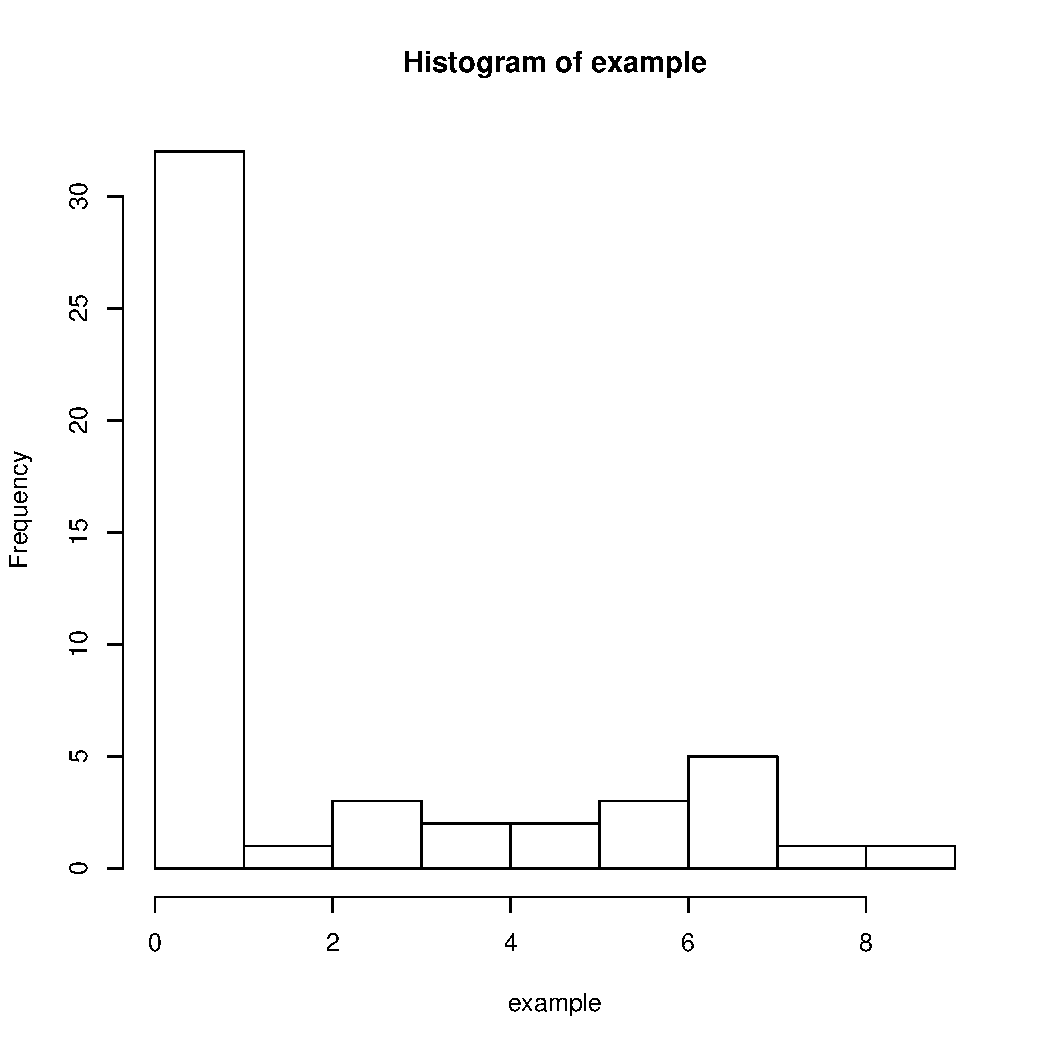
\includegraphics[width=50mm, height=50mm]{code/univariate_data_histogram.pdf}
% Density
\end{frame}

% 3. Univariate model
\begin{frame}
\frametitle{Univariate model formulation}

We start by building a relatively simple zero-inflated count model. Suppose that we observe
$$
X_i = R_i Y_i, \quad 1\le i\le n,
$$

\noindent where for $1\le i\le n$,
\begin{align*} 
R_i &\sim \text{Bernoulli}(\rho) \\
Y_i &\sim \text{Poisson}(\lambda)
\end{align*}

\noindent for parameters $\rho$ and $\lambda$,
but we do not observe $R_i$ or $Y_i$ themselves.
Being Bayesians we use the priors:
\begin{align*} 
\rho &\sim \text{Beta}(a_\rho, b_\rho) \\
\lambda &\sim \text{Gamma}(a_\lambda, b_\lambda).
\end{align*}

\end{frame}

% 5. How to fit, and advantages and disadvantages of each approach
% - Maximum likelihood
% - MCMC
% - VB

\begin{frame}
\frametitle{Comparison of fitting techniques}
\begin{tabular}{p{2cm}p{3.5cm}p{4.5cm}}
Technique & Pro & Con \\
\hline
MLE & EM could be used to fit these models, with $R_i$ as latent data & Not flexible to complications. \\
& & \\ %Frequentist \\
\hline
MCMC & Bayesian & Slow \\
	& Very accurate &  \\
\hline
Variational Bayes & Bayesian & May lose accuracy, or underestimate variance \\
& Fast  & Solution may be intractable \\ 
& Still quite accurate & \\
\hline
\end{tabular}

\end{frame}

% 6. Overview of Variational Bayes
\begin{frame}
\frametitle{An overview of Variational Bayes}
\begin{itemize}
\item \emph{Idea:} Approximate the full posterior $p(\theta|\vx)$ with a simpler approximation $q(\theta)$.

\item Fit $q(\theta)$ to the data by minimising the KL divergence between $p(\theta|\vx)$ and $q(\theta)$.

\item Theory guarantees that $\log p(x)\ge 
\log \underline{p}(x;q)$ and that 
$$
\log \underline{p}(x;q) = \int q(\vtheta) \left\{ \frac{p(\vy,\vtheta)}{q(\vtheta)} \right\}
$$ 

\noindent will
increase with each iteration.

\item If you use conjugate priors, a factored approximation can be used, and mean field updates can be used on
each parameter in turn until convergence is reached.
\end{itemize}
\end{frame}

\begin{frame}
\frametitle{An overview of Variational Bayes - Continued}
% - Algorithm
We iteratively update the parameters of each approximate distribution
in turn until the lower bound of the approximation converges.

\bigskip 
This could be thought of as a generalisation of Expectation Maximisation, where each parameter is thought of as a latent
variable and estimated according to the expectations of the other parameters.
\end{frame}




% 7a. Variational Bayes solution to ZIP
% - q-densities
\begin{frame}
Choose a factored approximation of the form
$$
q(\theta) = q(\lambda) q(\rho) \prod_{i=1}^n q(r_i)
$$
where
\begin{align*}
q(\lambda) &= \text{Gamma}(\alpha_{q(\lambda)}, \beta_{q(\lambda)}) \\
q(\rho) &= \text{Beta}(\alpha_{q(\rho)}, \beta_{q(\rho)}) \\
q(r_i) &= \text{Bernoulli}(p_i)
\end{align*}

% \begin{align*}
% q(\lambda) = \text{Gamma}(a_{\lambda_*}, b_{\lambda_*}) \\
% q(\rho) = \text{Beta}(a_{q(\rho)}, b_{q(\rho)}) \\
% q(r_i) = \text{Bernoulli}(p_i)
% \end{align*}

% - Algorithm
We iteratively update the parameters of each approximate distribution
in turn until the lower bound of the approximation converges.

\end{frame}
 

% 8. Results
% - Lower bound convergence
% - Accuracies
% 7b. Define accuracy
\begin{frame}
\frametitle{Mean field updates}
As we are using conjugate priors in our model, the mean field updates can be derived.
\begin{align*}
q(\lambda) &= \text{Gamma}(\alpha_{q(\lambda)} = \alpha_\lambda + \vone^T \vx, \beta_{q(\lambda)} = \beta_\lambda + \vone^T\vp) \\
q(\rho) &= \text{Beta}(\alpha_{q(\rho)} = \alpha_\rho + \vone^T\vr, \beta_{q(\rho)} = \beta_\rho + \vone^T(\vone - \vr)) \\
q(r_i) &= \text{Bernoulli}(p_i = \text{expit}(\eta_i))
\end{align*}
where
$$
\eta_i = - \frac{\alpha_{q(\lambda)}}{\beta_{q(\lambda)}} + \Psi(\alpha_{q(\rho)}) - \Psi(\beta_{q(\rho)})
$$

\end{frame}

\begin{frame}
\frametitle{Results/Accuracy}
% Definition of accuracy
Accuracy is defined as 1 minus half the difference in $L_1$ norm between the
true posterior distribution and the approximate posterior distribution of the
variational approximation.

$$
\text{Accuracy} = 1 - \half \|p(\vtheta|\vx) - q(\vtheta)\|_1
$$

This was calculated using the kernel density estimate of the posterior
distribution from MCMC minus the approximating distribution for each parameter of
interest.

\bigskip 
There was excellent accuracy for the univariate approximation, over 99\% in all of the cases that I looked at.
% Graph of lower bound
%\includegraphics{univariate_lower_bound_convergence.pdf}
\end{frame}

% 9. Extension to linear model
% 10. Overview GVA
% 11. Algorithm
% 12. Results?
% 13. What next
% 14. Conclusion
% 15. References
\begin{frame}
\frametitle{Extension to multivariate/regression models}
\begin{itemize}
\item Univariate models are a nice proof of concept.
\item Most applied statisticians want to build regression models.
\item Applied statisticians love mixed models.
\item There is a need for better approaches to fitting zero-inflated mixed models.
\item For example, MCMC with existing software can take \sout{minutes}hours 
to days to converge, or not converge at all.
\item That might not sound so bad to you, but how do you
do model selection? Applied statisticians and biostatisticians rarely know the true model.
\end{itemize}
\end{frame}



\begin{frame}
\frametitle{Linear mixed model set-up}
Let $\vone$ be a vector of 1s, and $\vone_n$ be a vector of 1s of
length n.

Consider a linear random intercept model with
$$
\begin{array}{ll}
\vy|\vbeta,\vu,\sigma_y^2 &\sim N(\mX \vbeta + \mZ \vu, \sigma_y^2 \mI) \\
\vbeta &\sim N(\vzero, \sigma_\vbeta^2 \mI) \\
\vu|\sigma_u^2 &\sim N(\vzero, \sigma_u^2 \mI)
\end{array}
$$
\noindent where
$$
\begin{array}{ll}
\vy & =
\begin{pmatrix}
y_1 \\
\vdots \\
y_n
\end{pmatrix} \\
\mX &= [\vone_n, \vx_1, \cdots, \vx_p] \\
\mZ &=
\begin{bmatrix}
\vone_{n_1} &  & \\
& \ddots & \\
& & \vone_{n_m}
\end{bmatrix} \\
\mC &= [\mX, \mZ]
\end{array}
$$
\end{frame}



\begin{frame}
\frametitle{Multivariate model formulation}
We use a zero-inflated Poisson random effects model.

\medskip

Suppose that we observe a vector of responses $\vy$ of length n, and matrices
of covariates $\mX$ and $\mZ$ of dimensions $n \times p$ and $n \times m$,
respectively.

\begin{align*}
p(\vy|\vbeta, \vu, \vr) &= \exp{(\vy^T\mR(\mX \vbeta + \mZ \vu) - \vr^Te^{\mX \vbeta + \mZ \vu} - \vone^T\log{(\vy !)})} \\
r_i|\rho & \stackrel{\mbox{\tiny iid}}{\sim} \text{Bernoulli}(\rho), \ \{i \colon y_i=0\} \\
\vu|\sigma_u^2 &\sim N({\bf 0}, \sigma_u^2 \mI) \\
\end{align*}
\noindent where $\mR =\mbox{diag}(\vr)$.
We use the priors:
\begin{align*}
\vbeta &\sim N({\bf 0}, \sigma_\vbeta^2\mI) \\
\sigma_u^2 &\sim IG(\alpha_{\sigma_u^2}, \beta_{\sigma_u^2}) \\
\rho &\sim \text{Beta}(a_\rho, b_\rho) \\
\end{align*}
\end{frame}

\begin{frame}
\frametitle{Form of the multivariate approximation}
We choose an approximation of the form
$$
q(\theta) = q(\vbeta, \vu) q(\sigma_u^2) q(\rho) \prod_{i=1}^n q(r_i)
$$
where
\begin{align*}
q(\vbeta, \vu) &\sim N(\vmu, \mLambda) \\
q(\sigma_u^2) &\sim IG(\alpha_{\sigma_u^2}, \beta_{\sigma_u^2}) \\
q(\rho) &= \text{Beta}(\alpha_{q(\rho)}, \beta_{q(\rho)}) \\
q(r_i) &= \text{Bernoulli}(p_i), \ \ 1 \leq i \leq n
\end{align*}
\end{frame}

\begin{frame}
\frametitle{Gaussian and Laplacian Variational Approximations}
\begin{itemize}
\item Lack of conjugacy means mean field updates won't be analytically tractable for the regression parameters.
\item We try Laplacian and Gaussian Variational Approximations instead, assuming that
$$
\begin{pmatrix}
\vbeta \\
\vu
\end{pmatrix}
\sim N(\vmu, \mLambda)
$$
and approximate as closely as we can.
\item For each iteration, we optimise to find
$\begin{pmatrix}
\vbeta \\
\vu
\end{pmatrix}
$ and $\mLambda$,
and then perform mean field updates on the other parameters.
\end{itemize}
\end{frame}

\begin{frame}
\frametitle{Mean field updates}
\begin{align*}
q(\vbeta, \vu) &= N(\vmu, \mLambda) \\
q(\sigma_{\vu}^2) &= IG\left(\alpha_{q(\sigma_{\vu}^2)} = \alpha_{\sigma_u^2} + \frac{m}{2}, \beta_{q(\sigma_{\vu}^2)} = \beta_{\sigma_u^2} + \frac{\|\vmu_\vu\|^2}{2} + \frac{\text{tr}(\mLambda_{\vu\vu})}{2}\right) \\
q(\rho) &= \text{Beta}(\alpha_{q(\rho)} = \alpha_\rho + \vone^T\vp, \beta_{q(\rho)} = \beta_\rho + \vone^T(\vone - \vp)) \\
q(r_i) & \sim \text{Bernoulli}{(p_i)}, \ \ \ 1 \leq i \leq n
\end{align*}
where
$$
p_i = \expit{\left [\Psi{(\alpha_{q(\rho)})} - \Psi{(\beta_{q(\rho)})} - \exp{\left(c_i^T\vmu + \half c_i^T \mLambda c_i\right)} \right ]}.
$$
\end{frame}

%\begin{frame}
%\frametitle{Progress so far}
%\begin{itemize}
%\item Computation - a work in progress. The multivariate model is
%implemented by combining my univariate VB code with John's GVA code.
%\item Initial signs are that this approach will work.
%\item The correct parameters are estimated for simulated test cases
%that we have tried.
%\item I've calculated the lower bound, but have not yet checked that it
%always increases for my test cases.
%\item Accuracy will be assessed against the random walk Metropolis-Hastings approximation of the true posterior.
%\end{itemize}
%\end{frame}

%\begin{frame}
%\frametitle{What next?}
%\begin{itemize}
%\item Continue working on the multivariate approximation.
%\item Extensions - random slopes, splines, and measurement error can all be 
%accomodated within a mixed model framework.
%\item Check accuracy against random walk Metropolis-Hastings approximation
%of the true posterior.
%\item Apply the mixed model fitting code to my physical activity data.
%\item Write this all up into a paper.
%\item Release an R package.
%\end{itemize}
%\end{frame}


%\begin{frame}
%\frametitle{Gaussian variational approximation}
%% Details from last time: Gaussian variational approximation
%For generalised linear models, there is no tractable factored 
%approximation which works well, so we attempt to approximate
%the GLM with a multivariate Gaussian (reference relevant
%Ormerod paper).
%\end{frame}

\begin{frame}
\frametitle{Laplacian approximation}
We Taylor expand the log likelihood $\log{p(\vtheta)}$ around the mode
$\vtheta_*$:
\begin{align*}
\log{p(\vtheta)} &\approx \log{p(\vtheta_*)} + \log{p'(\vtheta_*)}(\vtheta - \vtheta^*) + \half \log{p''(\vtheta_*)}(\vtheta - \vtheta^*)^2 \\
&= \log{p(\vtheta_*)} + \log{p''(\vtheta_*)}(\vtheta - \vtheta^*)^2
\end{align*}

as $\log{p^{'}(\vtheta_*)}(\vtheta - \vtheta^*) = 0$ at the mode. This has
the same form as a Gaussian density
\begin{align*}
\log{N(\vtheta|\vmu, \eta^{-1})} &= \half \log{\eta} - \frac{p}{2} \log{2 \pi} - \frac{\eta}{2} (\theta-\mu)^2 \\
&= \half \log{\frac{\eta}{2\pi}} + \half (-\eta)(\theta - \mu)^2
\end{align*}

and so we have an approximate posterior $q(\vtheta) = N(\theta|\mu, \eta^{-1})$ with
\begin{align*}
\mu &= \theta_* & \text{mode of the log-posterior, and}\\
\eta &= -\log{p''(\vtheta_*)} & \text{negative curvature at the mode.} \\
\end{align*}
\end{frame}

\begin{frame}
\frametitle{Optimising the Gaussian Variational Approximation}
The true likelihood $\log p(\vbeta, \vu, \mLambda)$ is hard to optimise due 
to the high dimensional integral involved, but the variational lower bound $\log \overline{p}(\vmu, \mLambda)$ can be optimised.
\begin{align*}
\log p(\vbeta, \vu, \mLambda) &= \vy^T \mR \mC \vnu + \vone^T c(\vy) + \frac{m}{2} \log |\mLambda| - \frac{mK}{2} \log{(2 \pi)}\\
&\quad + \log  \int_{\mathbb{R}^{m}} \exp \big[ \vy^T (\mR \mZ \vu - \mR^T b( \mX \vbeta + \mZ \vu)) \\
 &\quad \quad \quad \quad \quad \quad \quad - \half {\vu^T \mLambda^{-1} \vu } \big] d \vu + \text{const.}\\
\log \overline{p}(\vmu, \mLambda) &= \vy^T \mR \mC \vmu - \vp^T \exp{\left(\mC \vmu + \half \diag{(\mC \mLambda \mC^T)}\right)} \\
& \quad - \vmu^T \mSigma^{-1} \vmu - \half \tr{(\mLambda \mSigma^{-1})} + \half \log{|\mSigma^{-1}\mLambda|} + \text{const.} \\
%&= \mR\mC^T(\vy - B^{(1)}(\vmu, \sigma^2_u)) \\
%& \quad - \vmu^T \mSigma^{-1} \vmu - \half \tr{(\mLambda \mSigma^{-1})} + \half \log{|\mSigma^{-1}\mLambda|} + \text{const.} \\
\end{align*}
%\end{align*}
\end{frame}

\begin{frame}
\frametitle{Algorithms to fit model using GVA}
% Detail what progress has been made, and what results have been obtained
There are several alternative algorithms we've implemented or will implement
to fit this model:
% Point out the advantages of each
\begin{enumerate}
\item Optimise variational lower bound with L-BFGS, $\mLambda = \mR \mR^T$.\\
\quad Advantage: Accurate.
\item Optimise variational lower bound with L-BFGS, $\mLambda = (\mR \mR^T)^{-1}$. \\
\quad Advantage: Accurate, and very fast.
\item Newton-Raphson optimisation on the variational lower bound. \\
\quad Advantage: Straightforward to implement.
\item Newton-Raphson optimisation on the variational lower bound, using block inverses. \\
\quad Advantage: Straightforward to implement, and can be made fast.
\end{enumerate}

These algorithms should all fit the same model to the same data
within numerical tolerances.
\end{frame}

\begin{frame}
\frametitle{Cholesky factors}
Any symmetric matrix $\mSigma$ can be written $\mSigma = \mR \mR^T$
where $\mR$ is lower triangular. $\mR$ is unique if $\mR_{ii} \geq 0$.

\begin{align*}
&\begin{pmatrix}
\mR_{11} & 0 & 0 \\
\mR_{21} & \mR_{22} & 0 \\
\mR_{31} & \mR_{32} & \mR_{33}
\end{pmatrix}
\begin{pmatrix}
\mR_{11} & \mR_{21} & \mR_{31} \\
0 & \mR_{22} & \mR_{32} \\
0 & 0 & \mR_{33}
\end{pmatrix}
\\
=& \begin{pmatrix}
\mR_{11}^2 & & \text{symmetric}\\
\mR_{21}\mR_{11} & \mR_{21}^2 + \mR_{22}^2 \\
\mR_{31} \mR_{11} & \mR_{31}\mR_{21} + \mR_{32}L_{22} & \mR_{31}^2 + \mR_{32} ^2 + \mR_{33}^2
\end{pmatrix}
\end{align*}

So we only have $\frac{p(p-1)}{2}$ numbers to deal with instead of
$p^2$ numbers.

\end{frame}

\begin{frame}
% Motivations behind the algorithms
\frametitle{Motivations behind the algorithms}
% ii) The Cholesky factor of a block matrix of the form
% diag for random effects, block for cross effects
% block for cross effects, diag for fixed effects
% is mostly diagonal
% Less parameters to optimise and store
If we re-arrange the covariance matrix to have random effects before
fixed effects, our posterior covariance matrix is of the form
\begin{align*} \mLambda =
\begin{pmatrix}
\sigma_\vu^2 & 0 & \ldots & 0 & \sigma_{\vbeta \vu} & \sigma_{\vbeta \vu} \\
0 & \sigma_{\vu}^2 & 0 & 0 & \vdots & \vdots \\
\vdots & 0 & \ddots & 0 & \vdots & \vdots \\
0 & 0 & \ldots & \sigma_\vu^2 & \sigma_{\vbeta \vu} & \sigma_{\vbeta \vu} \\
\sigma_{\vbeta \vu} & \ldots & \ldots & \sigma_{\vbeta \vu} & \sigma_\vbeta^2 & 0 \\
\sigma_{\vbeta \vu} & \ldots & \ldots &\sigma_{\vbeta \vu}  & 0 & \sigma_\vbeta^2
\end{pmatrix}
\end{align*}

As the $\sigma_\vu^2$ block is diagonal, the Cholesky factor is 
sparse, with only $m + \frac{p(p-1)}{2}$ non-zero elements. If $p$ is small
and $m$ is large, as will typically be the case, then this algorithm will
be much faster.

\end{frame}

\begin{frame}
\frametitle{Implementation}
% Work to date
\begin{itemize}
\item We've written 2,000 lines of R code, about enough for an R package.
\item There are 93 functions so far.
\item I spend my life debugging this code.
\item I've had to learn some numerics/computational statistics along the
way.
\item There's still plenty to do \ldots
\end{itemize}
\end{frame}

\begin{frame}
\frametitle{Accuracy results using MCMC}
\begin{itemize}
\item Accuracy verified using 1 million MCMC iterations from Stan.
\item Stan converts your model specification into C++ code.
\item A one million iteration run for this model took over 32 CPU days.
\item Stan can be parallelised across multiple cores.
\item Pro tips:
\begin{itemize}
\item Check your computer has enough RAM.
\item Run longrunning tasks with R -f script.R and nohup.
\item Run them on the biggest, fastest server you can find. verona's pretty good.
\item Checkpoint every few thousand iterations.
\end{itemize}
\item The need for approximate methods is obvious, this is simply not
practical for many types of applied work.
\end{itemize}
\end{frame}

\begin{frame}
\frametitle{Accuracy results}
\begin{tabular}{ccccc}
\hline
	& Laplacian & GVA $(\mLambda=\mR \mR^T)$ & GVA $\mLambda=(\mR \mR)^{-1}$ & GVA NR \\
\hline
$\vbeta_1$&0.95&0.95&0.95&0.95 \\
$\vbeta_2$&0.81&0.90&0.85&0.90 \\
$\vu_1$&0.95&0.96&0.95&0.96 \\
$\vu_2$&0.94&0.96&0.94&0.96 \\
$\vu_3$&0.95&0.96&0.95&0.96 \\
$\vu_4$&0.95&0.96&0.95&0.96 \\
$\vu_5$&0.95&0.96&0.95&0.96 \\
$\vu_6$&0.95&0.96&0.95&0.96 \\
$\vu_7$&0.94&0.95&0.95&0.95 \\
$\vu_8$&0.95&0.96&0.95&0.96 \\
$\vu_9$&0.92&0.94&0.93&0.94 \\
$\vu_{10}$&0.95&0.97&0.95&0.97 \\
$\sigma_\vu^2$&0.96&0.95&0.96&0.95 \\
$\rho$&0.90&0.90&0.90&0.90 \\
\hline
\end{tabular}
\end{frame}

% Pretty pictures
\begin{frame}
\frametitle{Plots of the MCMC-estimated and approximating densities}
\end{frame}

\begin{frame}
\frametitle{Further work}
\begin{itemize}
\item All algorithms should arrive at exactly the same result, up to numerical error i.e. around $10^{-4}$. But they currently don't.
\item More checking. These algorithms should produce the same results on
a wide range of randomly generated data sets.
\item Algorithms i and iii work well.
\item Algorithm ii is accurate on some data sets, but this isn't good enough.
\item I have concerns about its stability.
\item Algorithm iv is yet to be implemented, but should be straightforward.
\item Splines should be ``easy'' to implement. Doesn't require any major changes to the existing code.
\item Finish writing this all up into a paper, and release an R package.
\end{itemize}
\end{frame}

\begin{frame}
\frametitle{References}
\begin{itemize}
\item Explaining Variational Approximations, J.T. Ormerod, M.P. Wand, American Statistician, 2010
\item Gaussian Variational Approximations, J.T. Ormerod, M.P. Wand, 2012
\item General Design Mixed Models, M.P. Wand and others, 2006
\end{itemize}
\end{frame}

\end{document}
